% Chapter 4

\chapter{Architecture}

\label{ch:architecture}

%----------------------------------------------------------------------------------------

\section{Overview}\label{sec:overview}

\tangible{} is implemented as a single Python package, without any external
dependencies.

The architecture of \tangible{} can be categorized into four different parts: The
\hyperref[sec:ast]{abstract syntax tree (AST)}, \hyperref[sec:backends]{code
generation backends}, \hyperref[sec:shapes]{shapes} and
\hyperref[sec:utils]{utils}.

\vspace{7mm}

\begin{figure}[H]
	\centering
	\definecolor{BackendsColor}{RGB}{116,143,204}
\definecolor{AstColor}{RGB}{199,108,107}
\definecolor{ShapesColor}{RGB}{227,225,107}
\definecolor{UtilsColor}{RGB}{118,219,125}

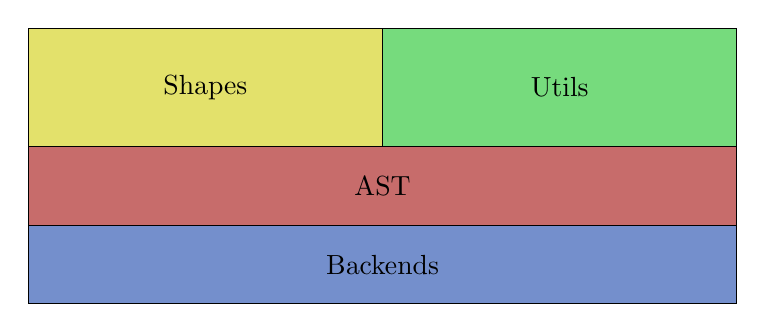
\begin{tikzpicture}
	\filldraw [fill=BackendsColor] (0,0) rectangle node [align=center] {Backends} (9,1) ;
	\filldraw [fill=AstColor] (0,1) rectangle node [align=center] {AST} (9,2);
	\filldraw [fill=ShapesColor] (0,2) rectangle node [align=center] {Shapes} (4.5,3.5);
	\filldraw [fill=UtilsColor] (4.5,2) rectangle node [align=center] {Utils} (9,3.5);
\end{tikzpicture}

	\caption{Architecture Diagram}
	\label{img:architecture}
\end{figure}

%----------------------------------------------------------------------------------------

\section{AST}\label{sec:ast}

The \texttt{ast.py} module provides the objects for the abstract syntax tree
(AST) for \tangible{}. All AST objects extend a single base class called
\texttt{AST}. This base class is responsible for three things:

\begin{itemize}
	\item It provides a single base type to use for type checking, e.g.
		\texttt{isinstance(mysubclass, ast.AST)}.
	\item It overrides the \texttt{\_\_eq\_\_} and \texttt{\_\_ne\_\_} methods in
		a way that all subclasses are compared by value (using
		\texttt{self.\_\_dict\_\_}), and not by identity.
	\item It provides a \texttt{\_\_repr\_\_} implementation that displays both
		the class name as well as the object memory address, which simplifies
		debugging.
\end{itemize}

\noindent The module contains the following classes:

\subsection{Base Class}

\begin{itemize}
	\item \texttt{AST}: The base shape for all AST elements, as described above.
\end{itemize}

\subsection{2D Shapes}

\begin{itemize}
	\item \texttt{Circle}: A circle shape with a specified radius.
	\item \texttt{CircleSector}: A circle sector shape (pizza slice) with a
		specified radius and angle.
	\item \texttt{Rectangle}: A rectangular shape with a specified width and
		height.
	\item \texttt{Polygon}: A polygon shape made from a list of 2D coordinates.
\end{itemize}

\subsection{3D Shapes}

\begin{itemize}
	\item \texttt{Cube}: A cube with a specified width, height and depth.
	\item \texttt{Sphere}: A sphere with a specified radius.
	\item \texttt{Cylinder}: A cylinder with a height and top/bottom radii.
	\item \texttt{Polyhedron}: An arbitrary 3D shape made from connected triangles
		or quads.
\end{itemize}

\subsection{Transformations}

\begin{itemize}
	\item \texttt{Translate}: Used to translate an object.
	\item \texttt{Rotate}: Used to rotate an object.
	\item \texttt{Scale}: Used to scale an object.
	\item \texttt{Mirror}: Used to mirror an object.
\end{itemize}

\subsection{Boolean Operations}

\begin{itemize}
	\item \texttt{Union}: Combine multiple shapes into a single shape.
	\item \texttt{Difference}: A boolean difference of two or more shapes.
	\item \texttt{Intersection}: A boolean intersection of two or more shapes.
\end{itemize}

\subsection{Extrusions}

\begin{itemize}
	\item \texttt{LinearExtrusion}: Extrude a 2D object linearly along the z axis.
	\item \texttt{RotateExtrusion}: Extrude a 2D object around the z axis. 
\end{itemize}

%----------------------------------------------------------------------------------------

\section{Backends}\label{sec:backends}

The backends are responsible for code generation. They receive an
\hyperref[sec:ast]{AST} instance, traverse it and emit backend specific code.

At the time of this writing, only one backend has been implemented: The OpenSCAD
backend. But it's be very easy to add additional backends in the future.

\subsection{Creating Custom Backends}

To be valid, a custom backend simply needs to implement the following interface:

\vspace{.5\baselineskip}

\begin{pythoncode}
class CustomBackend(object):
    def __init__(self, ast):
        """Initialize backend using the provided AST."""
    def generate(self):
        """Generate code from AST and return it
        as a unicode string."""
\end{pythoncode}

\noindent The code generated by a backend is returned as a unicode string. It
can then be printed to the terminal or used for further processing.


TODO: cross-reference to implementation details

%----------------------------------------------------------------------------------------

\section{Shapes}\label{sec:shapes}

The \texttt{shapes} package is a key component of \tangible{}. It provides a
hierarchical collection of pre-defined shapes that can be used directly to
generate three dimensional data visualizations.

The package is organized into different files:

\begin{itemize}
	\item \texttt{base.py}: Base class for all shape objects.
	\item \texttt{mixins.py}: Mixins used in the shape classes, mostly used for
		data validation.
	\item \texttt{bars.py}: Bar like shapes.
	\item \texttt{vertical.py}: Vertical shapes, e.g. towers.
	\item \texttt{pie.py}: Circular "pie" shapes.
\end{itemize}

\begin{figure}[H]
	\centering
	\definecolor{ShapesColor}{RGB}{227,225,107}

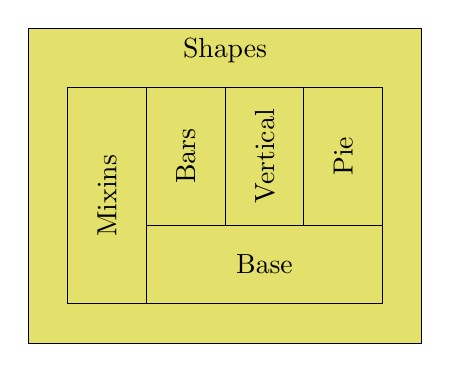
\begin{tikzpicture}

	% Main rectangles

	\filldraw [fill=ShapesColor] (0,0) rectangle (5,4);

	% Inner rectangles

	\draw (1.5,0.5) rectangle node {Base} (4.5,1.5);
	\draw (1.5,1.5) rectangle node [rotate=90] {Bars} (2.5,3.25);
	\draw (2.5,1.5) rectangle node [rotate=90] {Vertical} (3.5,3.25);
	\draw (3.5,1.5) rectangle node [rotate=90] {Pie} (4.5,3.25);
	\draw (0.5,0.5) rectangle node [rotate=90] {Mixins} (1.5,3.25);

	% Labels

	\node [below] at (2.5,4) {Shapes};

\end{tikzpicture}

	\caption{Shapes Architecture}
	\label{img:shapes}
\end{figure}

\subsection{Base Class}

The class \texttt{Shape} in \texttt{shapes/base.py} is the base class for all
predefined shapes in \tangible{}:

\vspace{.5\baselineskip}

\begin{pythoncode}
class BaseShape(object):
    def _build_ast(self):
        raise NotImplementedError("_build_ast method not implemented.")

    def render(self, backend):
        self.ast = self._build_ast()
        return backend(self.ast).generate()
    
class Shape(BaseShape):
    def __init__(self, data):
        self.data = utils.ensure_list_of_lists(data)
        if len(self.data[0]) == 0:
            raise ValueError("Data may not be empty.")
\end{pythoncode}

Each shape is initialized with the data as the first positional argument. Using
a helper function, single lists with one dimensional data are converted to
nested lists, to simplify the rendering code. Empty data is not allowed.

The \texttt{\_build\_ast()} method is not implemented in the base class. An
inheriting class needs to override the method and return an AST.

Finally, the \texttt{render(backend)} method renders the AST using the specified
backend class and returns the resulting source code as a unicode string.

\subsection{Mixins}

The mixin classes are used in combination with Python's multiple inheritance
system to provide "pluggable" generic data validation. At the time of this
writing, the following mixins are available:

\begin{itemize}
	\item \texttt{Data1DMixin}: Ensures that data contains exactly 1 dataset.
	\item \texttt{Data2DMixin}: Ensures that data contains exactly 2 datasets.
	\item \texttt{Data4DMixin}: Ensures that data contains exactly 4 datasets.
	\item \texttt{DataNDMixin}: Used for shapes where the number of data
		dimensions is not relevant. But it asserts that the data is not empty and
		that all data items are of a sequence type.
	\item \texttt{SameLengthDatasetMixin}: Ensures that all datasets have the same
		length.
\end{itemize}

The mixins are properly implemented using Python's argument list unpacking
(\texttt{\textsuperscript{*}args, \textsuperscript{**}kwargs}) and
\texttt{super()} calls, so that a class can use multiple mixins without breaking
.the inheritance chain. A good example where this is used is the
\texttt{RectangleTower2D} shape:

\vspace{.5\baselineskip}

\begin{pythoncode}
class RectangleTower2D(Data2DMixin,
    SameLengthDatasetMixin, VerticalShape):
    # ...
\end{pythoncode}

\subsection{Shape Classes}

\tangible{} provides different shapes ready to use. They are grouped into three
categories: Bar shapes, vertical shapes and  pie shapes.

\begin{itemize}
	\item Bar shapes consist of several bars that start on \texttt{z=0} and have a
		height depending on the corresponding datapoint. They can be aligned in
		rows, and rows can be combined to create 3D bar graphs.
	\item A vertical shape is a shape with layers stacked on top of each other,
		with a fixed layer height, for example a round tower where the radius
		corresponds to the datapoint.
	\item A pie shape can represent data as angle, height or radius of the
		corresponding slice. It is possible to define an inner radius ($\rightarrow$donut) and
		to explode the slices.
\end{itemize}

\noindent The naming of the shape classes follows a consistent pattern: First a
descriptive name of the shape (e.g. \texttt{RhombusTower} or
\texttt{RadiusHeightPie}), then the dimensionality of the data (e.g.
\texttt{1D}, \texttt{4D} or \texttt{ND}). A way to describe the data
dimensionality in Python terms would be \emph{\texttt{n}-dimensional data is a
list containing \texttt{n} lists}.

TODO a separate chapter or section containing all shapes

%----------------------------------------------------------------------------------------

\section{Utils}\label{sec:utils}
